\documentclass[12pt, a4paper]{article}

%PACK------------------------------
\usepackage[utf8]{inputenc}
\usepackage[british, polish]{babel}
\usepackage{geometry}
\usepackage{gensymb} %pakiet symboli
\usepackage[upgreek, LGRgreek]{mathastext}
\usepackage{bm}
\usepackage{lipsum}
\usepackage{cite}
\usepackage{graphicx}
\usepackage{hyperref}
\usepackage{seqsplit}
\usepackage[monochrome]{xcolor}
\usepackage{mathptmx}
\usepackage{fontspec}

%SETTING---------------------------
%\defaultfontfeatures{LetterSpace=5}
\setmainfont{Times New Roman}
\setlength{\parindent}{0pt}
\setlength{\parskip}{0pt}
\linespread{1.25}
\geometry{left=2.54cm, right=2.54cm, top=2.54cm, bottom=2.54cm}
% \renewcommand{\thesection}{\arabic{section}.}
% \renewcommand{\thesubsection}{\thesection\arabic{subsection}.}
\newcommand*{\myfont}{\fontfamily{pcr}\selectfont}

%DOCUMENT--------------------------
\begin{document}
\begin{titlepage}
    \thispagestyle{empty}
    \begin{center}
    
        \textbf{\large Uniwersytet Jagielloński w Krakowie}
        
        \vspace{0.5cm}
        
        \textbf{\Large Wydział Biochemii, Biofizyki i Biotechnologii}
        
        \vspace{0.5cm}
        
        \begin{figure}[h]
            \centering
            \includegraphics[width=4cm]{figures/Herb_Uniwersytetu_Jagiellońskiego.svg.png}
            \label{fig:title}
        \end{figure}
        
        \vspace{0.5cm}

        \textbf{\huge Optymalizacja pomiarów napięcia w~układzie MFC z jednoczesną produkcją MlrA w komórkach \textit{Synechocystis sp.}}

        \vspace{2cm}

        {\Large Filip Stanisław Hajdyła}\\
        Nr albumu: 1164936

        \vspace{2cm}
        
        {\large Praca licencjacka z Biotechnologii}
        
        \vspace{0.5cm}
        
        {\large pod opieką dr hab. Dariusza Dzigi}
        
        \vspace{1cm}
        
        \textbf{\Large Pracownia Metabolomiki}
        
        \vspace{2cm}
        
        Kraków, 2022
        
    \end{center}
\end{titlepage}

\newpage

% \begin{flushright}
% strona na podziękowania (i jakieś łacińskie motto dla picu)
% \end{flushright}

\tableofcontents

\begin{abstract}
    \noindent
    \lipsum[1]
\end{abstract}

\rule{\textwidth}{0.4pt}

\begin{otherlanguage}{british}
    \begin{abstract}
        \noindent
        \lipsum[1] 
    \end{abstract}
\end{otherlanguage}

\section{Wstęp}\label{sec:intro}
MFC (\textit{ang.} Microbial Fuel Cell) to urządzenia umożliwiające generowanie energii elektrycznej z wykorzystaniem
mikroorganizmów.
Należą one do szerszej klasy urządzeń BES (\textit{ang.} Bio-Electrochemical Systems) \cite{}.
W ostatniej dekadzie zainteresowanie systemami BES, a w szczególności MFC wzrosło diametralnie, co odzwierciedla wzrost
liczby związanych z nimi publikacji, przedstawiony na rys.~\ref{fig:1}.
Pomysł wykorzystania mikroorganizmów do generowania elektryczności przypisuje się Michaelowi Potterowi~\cite{Potter1911},
natomiast idea ,,elektryczności zwierząt'', a więc elektryczności związanej z układami ożywionymi, sięga aż XVIII wieku.
W systemach MFC, do generowania elektryczności, wykorzystuje się utleniająco-redukujący charakter reakcji metabolicznych
przeprowadzanych przez mikroorganizmy, które możemy podzielić na rezydujące na powierzchni anody elektrogeny
(uwalniające elektrony) oraz zasiedlające katodę elektrotrofy (pobierające i wykorzystujące elektrony).


\begin{figure}[!b]
    \centering
    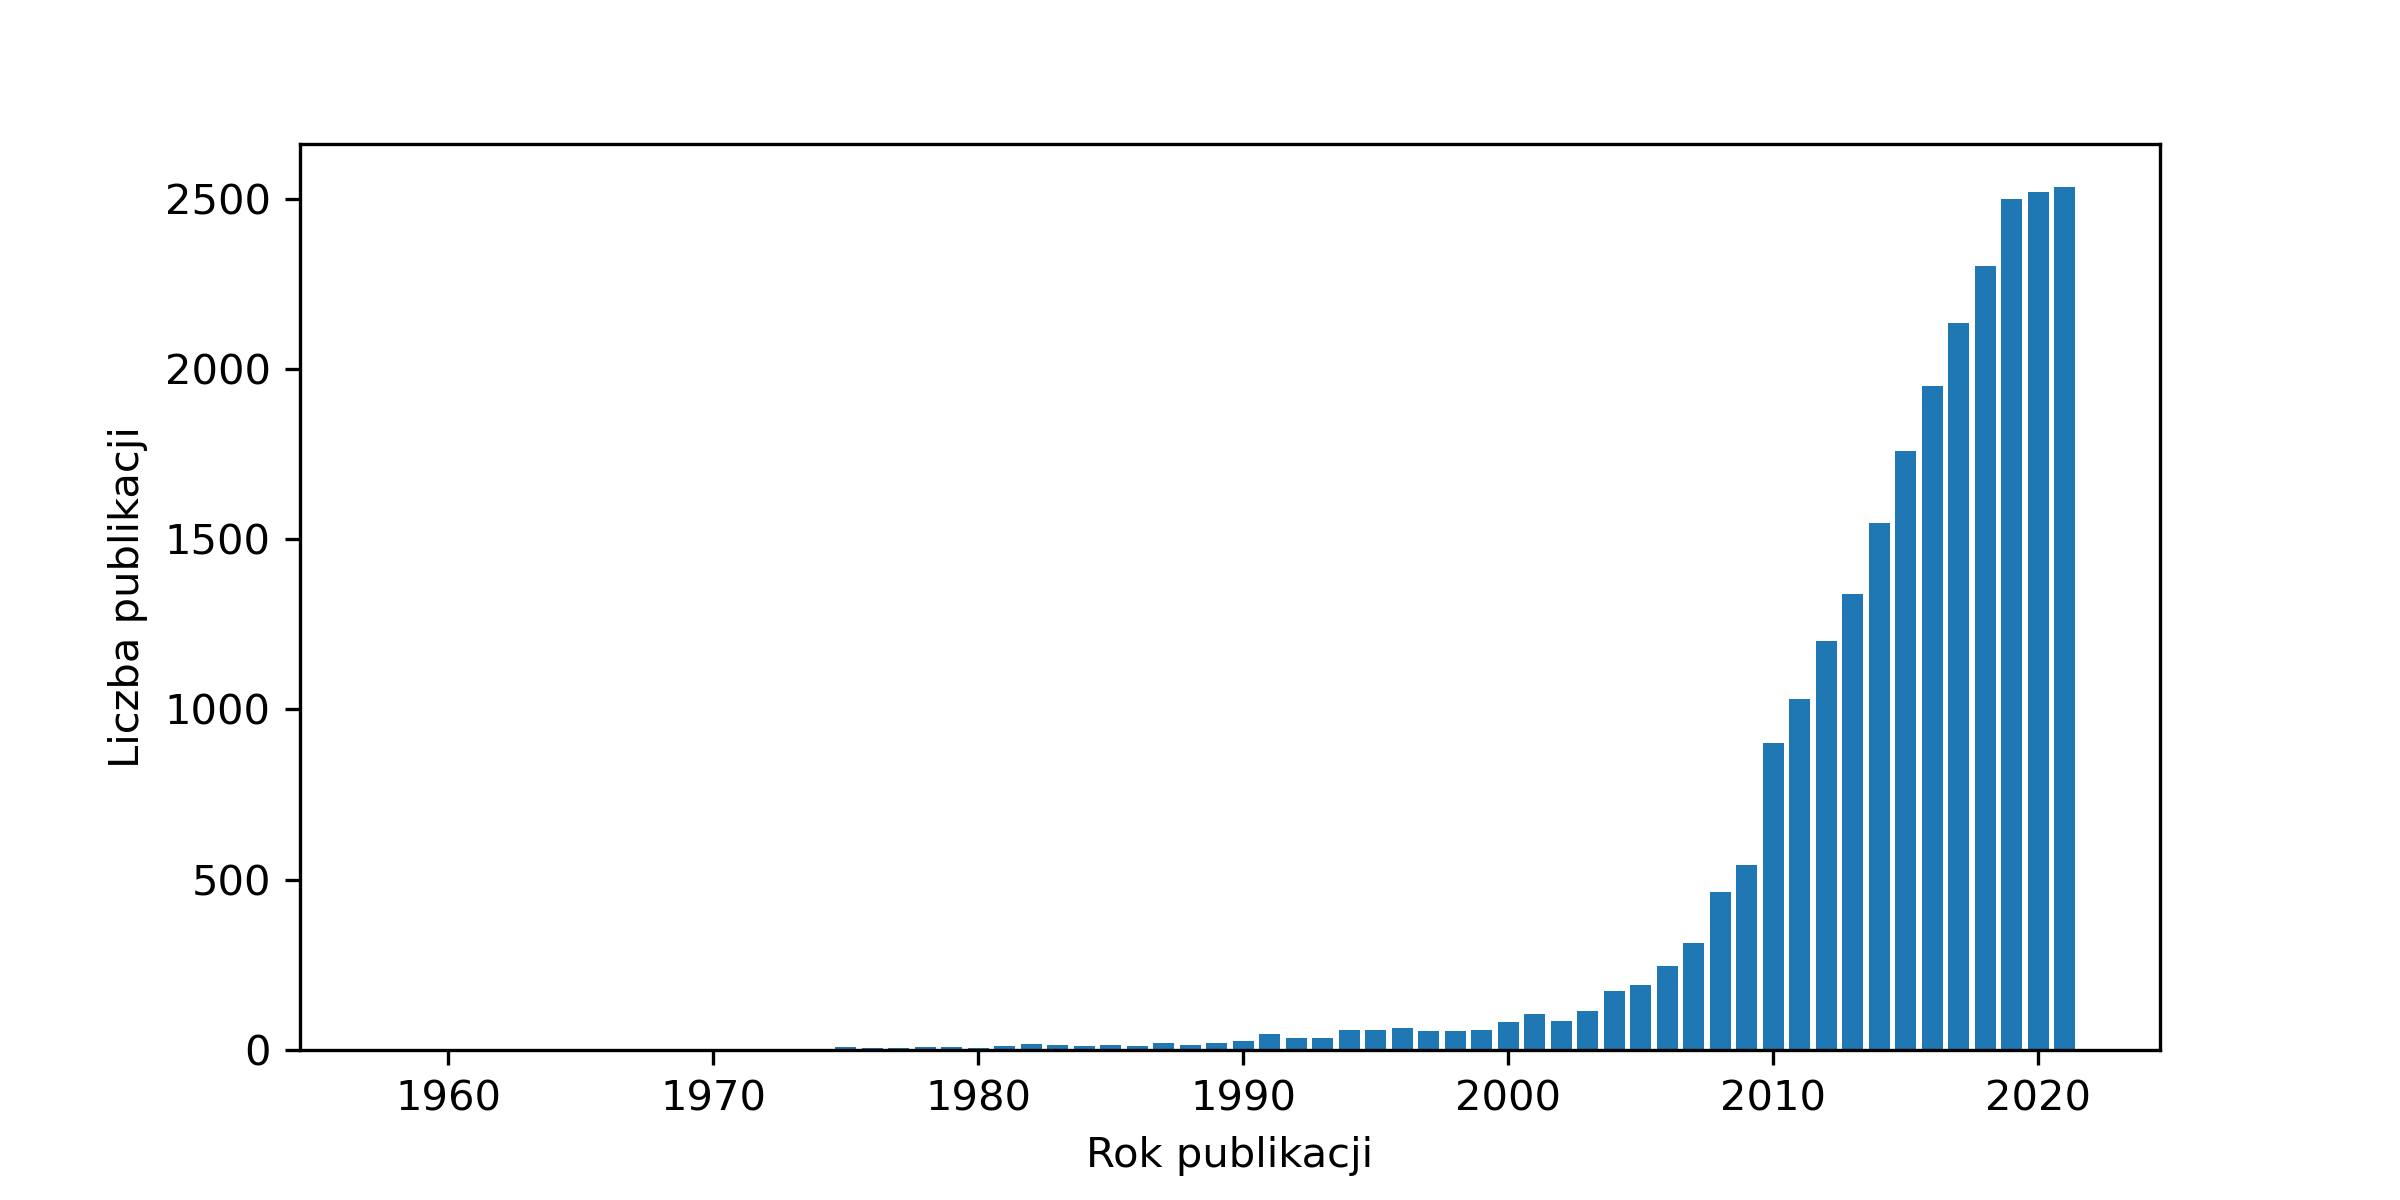
\includegraphics[width=\textwidth]{figures/pub}
    \caption{Liczba publikacji z ,,MFC'' lub ,,Microbial Fuel Cell'' w tytule w latach 1958--2021.}
    \label{fig:1}
\end{figure}

% \begin{figure}[t]
%     \centering
%     \includegraphics{}
%     \caption{Caption}
%     \label{fig:my_label}
% \end{figure}


\section{Metody}\label{sec:methods}
\subsection{metoda 1}
\lipsum[2]
\subsection{eksperyment uno}
\lipsum[3-5]

\section{Analiza Danych}\label{sec:analysis}
\subsection{dane}
\lipsum[2-4]
\subsection{więcej danych}
\lipsum[2-4]
\subsection{jeszcze więcej zasranych danych}
\lipsum[2-4]

\bibliographystyle{plain}
\bibliography{main}



\end{document}


